% #############################################################################
% This is Chapter 4
% !TEX root = ../main.tex
% #############################################################################
% Change the Name of the Chapter i the following line
\fancychapter{Evaluation}
%\cleardoublepage
\label{chap:evaluation}
 
This chapter focuses on the evaluation of the proposed framework, from different perspectives, which include the diversity of the algorithms currently supported by the solution's prototype, their performance, and the visual mechanisms. To this end, we divide the evaluation in two phases: in \Cref{sec:qualitative}, we discuss the qualitative properties of the current prototype, outlining the flexibility and heterogeneity of the provided algorithms, while in \Cref{sec:quantitative}, we assess the viability of the current prototype in the architectural practice by using it to address three real case studies. These case studies corroborate the suitability of the algorithmic framework described in\Cref{chap:implement}, by using the optimizer prototype and the Khepri \ac{AD} tool to enable the application of different optimization algorithms. 

Overall, this evaluation aims to answer the following questions: 
\begin{itemize}
	\item Do the studied algorithms present benefits for the architectural practice? Particularly, are they able to reduce the impact of the expensive performance analysis that are typically employed in building design?
	\item Is there any algorithm or class of algorithms that constantly outperforms others?
	\item Is there any difference between different \ac{MOO} approaches?
	\item Is the proposed framework applicable to the architectural practice? 
	\item ...\todo{Melhorar estas research paths...}
\end{itemize}

\section{Qualitative Evaluation}
\label{sec:qualitative}

The quantitative evaluation of optimization frameworks involve considering multiple aspects, including the flexibility, adaptability, diversity of algorithms, ease of use, among others. Calling upon the \acp{NFLT} discussed in \Cref{ssec:comparisondfo}, some algorithms are really good solvers for some problems and very poor solvers for others~\cite{Wolpert1997NFLT}. Selecting the right algorithm can have a great impact in the efficiency of optimization processes. Particularly, in building design, to benefit from such performance gains, diversity of algorithms allows to face each problems' characteristics differently, enabling the identification of most promising algorithms. In addition to the algorithms' diversity, in order to be easily used by less experienced users, algorithms should be effortlessly run, without the need for many manual changes. Notwithstanding their innate simplicity, optimization frameworks should also be flexible enough to enable more experienced users to fine-tune them according to their expertise, thus fostering more efficient optimization processes. At last, a good framework should adapt to handle different problems.

Regarding the adaptability of the current prototype, it provides mechanisms to address both single- and multi-objective problems: 15 \ac{SOO} algorithms and 13 \acp{MOEA}, respectively. Simpler approaches, like the design of experiments approach discussed in \Cref{ssec:doe}, are also possible using one of the 5 sampling methods available in the prototype. Moreover, a crucial features of this prototype is that it provides 10 \ac{ML} algorithms to be used with other techniques, thus allowing to reduce the time complexity involved in building design. 

\todo{Tabela / Imagem - discriminativa sobre os tipos de algoritmos e as classes}

\todo{Table X} presents a view of the algorithms supported by the prototype discriminated by class and domain. When comparing to currently existing tools in architecture, our solution presents a more extense and diverse set of algorithms, which can be explored to address a wider variety of problems. Moreover, while the existing tools rely on a unique optimization approach (e.g., \ac{SOO}, or Pareto-based optimization), our solution adapts to the user needs, providing the necessary mechanisms to the different approaches.

Unlike existing tools, which are implemented on top of visual programming languages, like Grasshopper and Dynamo, the prototype is implemented on top of a textual programming language. Although the graphical feel of the visual programming paradigm provides a more comfortable experience to less experienced users, the fact that the prototype makes use of the textual paradigm confers more scalability and portability to the achieved designs, thus allowing users to seamless apply optimization to more complex buildings. Nevertheless, to make it more appealing to less experienced users, the prototype includes a ready-to-use format, where every algorithm is configured by default.  

Besides the ready-to-use format, the prototype supports finer configurations of the different algorithms, thus allowing more experienced users to employ their knowledge to fine-tune and, if desired, to conjugante different algorithms. 

Moreover, given the importance of testing different algorithms before settling for a single one~\cite{Wortmann2016BBO}, the prototype provides the necessary mechanisms to facilitate and automate testing multiple algorithms with no additional efforts for the user. Conversely, existing architectural tools require the user's intervention in order to test different algorithms, eitherr by dragging other optimizer components and making necessary changes in the design script (e.g., ) or, when possible, by simply re-configuring the optimization tool to use one of the other supported algorithms. 

Regarding the post-processing and logging mechanisms, the proposed prototype is automatically configured to produce extensive log files, including all the information about the algorithms and problems being addressed, as well as a real-time log of the different solutions explored during the optimization run. This differs from existing tools, which only made the log files available in the end of the run. That being said, some of the currently existing tools still outperform the proposed prototype in terms of the visualization and interactivity features. The proposed prototype provides visual interactive Python scripts that read the log files and produce the corresponding plots. However, this plots are not updated in real time, instead requiring the user to re-run the script.

\todo{Comentar a facilidade c/ que alguém que já tem um programa AD consegue acopolar optimização a AD.}
% #############################################################################
\section{Quantitative Evaluation}
\label{sec:quantitative}

In order to study and explore the behavior of algorithms within building design domains, we evaluate the performance of different algorithms using the optimizer prototype,  discussed in \Cref{chap:implement}, to assess their performance in the context of building design problems. In order to evaluate the real applicability of the proposed framework, we tested our prototype in three case studies proposed by a small-scale architectural studio\footnote{Atelier dos Remédios}: (1) the optimization of the lighting conditions of a solarium in a private house in Portugal, (2) the optimization of the structural behavior and the elegance of an arc-shaped space frame structure for an arts exhibition pavillion, and (3) the optimization of the cost and the lighting conditions of an exhibition room in an arts pavillion.   

% #############################################################################
\subsection{Ericeira House: Solarium}

\begin{figure}
	\centering
	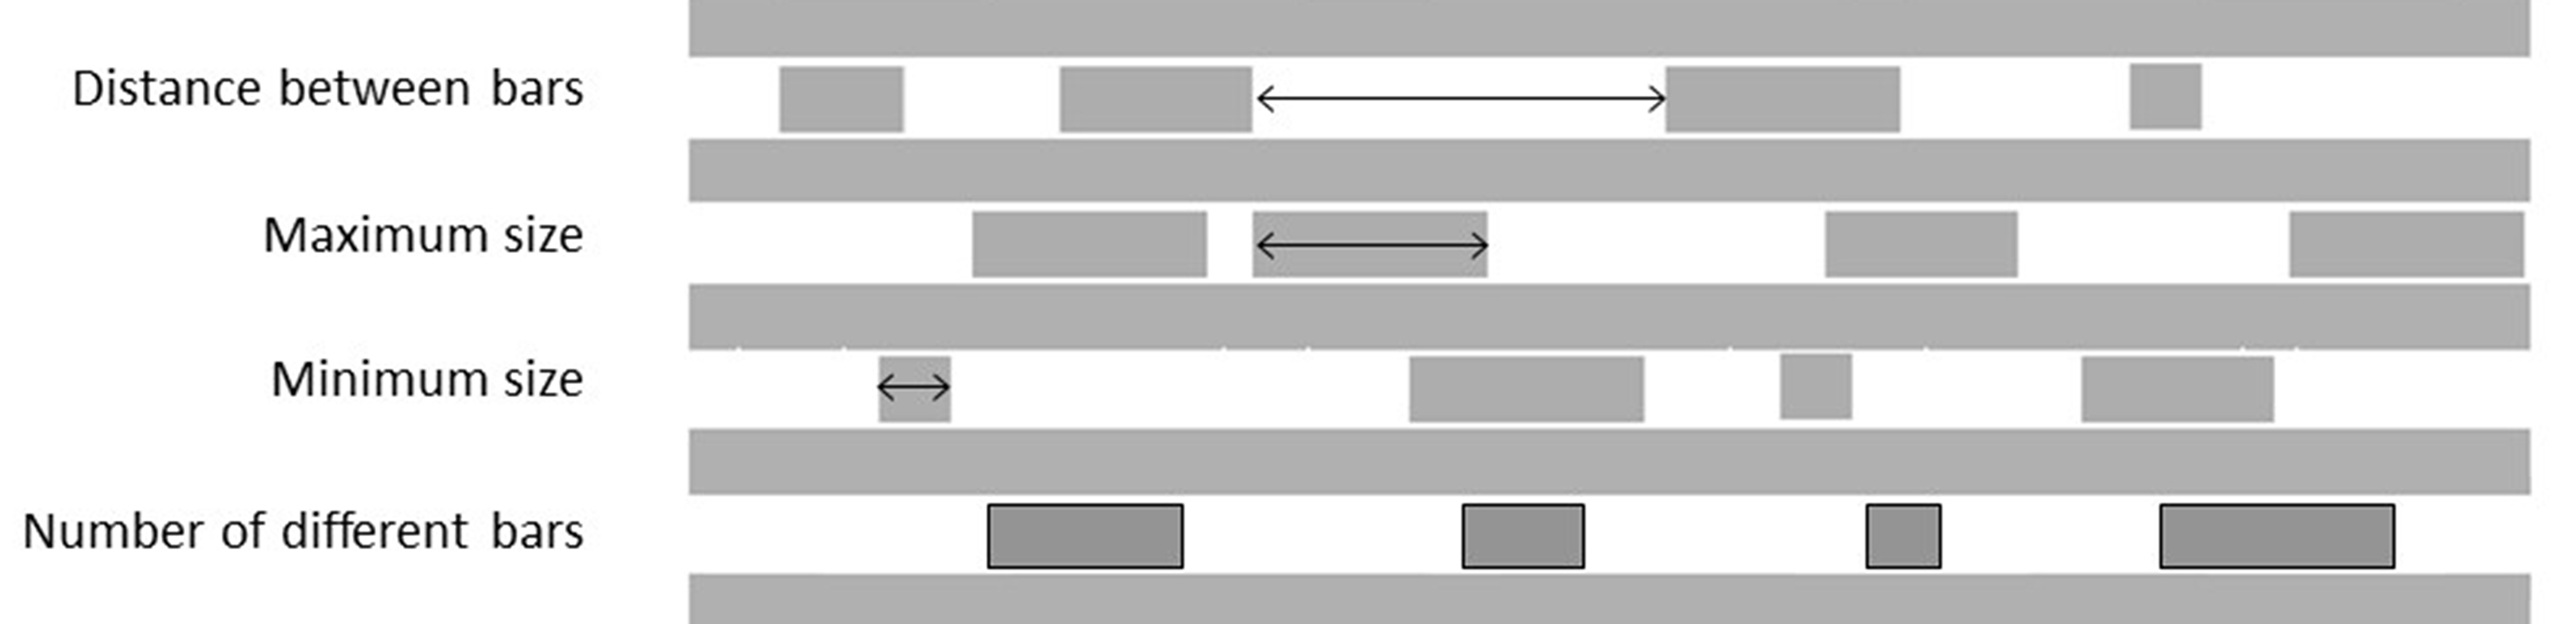
\includegraphics[width=\textwidth]{Images/Evaluation/Ericeira_1.jpg}
	\caption{Representation of the shading panels' geometric pattern and its design variables.}
	\label{fig:ericeira_panels_explanation}
\end{figure}

The first case study involves the optimization of the lighting conditions of a room in an isolated private house in Portugal~\cite{Caetano2018,Belem2018optimizeddesign}. The room was designed with a set of façade shading panels that modulate the daylight conditions on the interior of the room. Depicted in \Cref{fig:ericeira_panels_explanation}, the panels are composed of a set of horizontal wood bars of different sizes, which alternate between one full-length bar and a set of smaller bars. For aesthetics reasons, the size and position of the smaller bars along the panel's width were randomized. The final pattern of the façade's shading panels is thus defined in term of four variables, which were constrained by the architects to vary within certain values: the length’s step, the maximum distance separating two consecutive bars, and the minimum and maximum lengths of the smaller bars. The architects expressed interest in achieving a solution for the shading panels that was optimized in terms of its lighting performance, which was measured using a daylight metric \ac{sUDI}\todo{Nabil and Mardaljevic 2006}. Therefore, the goal was to maximize the \ac{sUDI} values that would give the best lighting performance for the private room. \Cref{fig:ericeira_multiple_panels} represents some variations of this case study with different \ac{sUDI} values.

\begin{figure}
	\centering
	\includegraphics[width=\textwidth]{Images/Evaluation/Ericeira_2.png}
	\caption{Representation of shading panels’ geometric pattern with different sUDI values (from left to right, 7\%, 62\%, 90\%, and 100\%).}
	\label{fig:ericeira_multiple_panels}
\end{figure}
%http://papers.cumincad.org/data/works/att/caadria2018\_278.pdf

\todo{
	- Falar do trabalho no primeiro paper:
	< Seguimos uma abordagem DoE, no qual aplicámos um processo iterativo que foi restringindo os bounds sucessivamente até obtermos uma amostra melhor}
The first approach to this case study~\cite{Caetano2018} followed a simple design of experiments approach, using two sampling algorithms to generate different design variations: Monte Carlo sampling and Latin hypercube sampling (see \Cref{chapter:appendixA}). In order to find an optimal solution, initially the architects suggested 
design space larger than the one suggested by the architects' the architects’ suggestions for the parameters, but also a larger design space that resulted from the assignment of values that deviated from those premise

The optimization process was then repeated, but this time considering theconstraint set by the architects of using stripes of 5, 10, 15, 20, or 25 cm length.Only the distance between each stripe (the variableD-max) was dictating the lightentering the room. We started by setting theD-maxvalue as 20 cm, like thearchitects had suggested, and we generated 50 samples, obtaining a maximumsUDIvalue of around 45\%, which was far from being optimum. Consequently,the optimization process was redone using, this time, aD-maxvalue of 100 cm,generating200samples. ThescatterplotinFigure2organizestheobtainedsample,demonstrating that, until reaching a maximum distance of 50cm, thesUDI rapidlyincreases to 80\%, whereas after that it slowly converges to 100\%. Nevertheless,most of the solutions corresponding to highersUDIvalues resulted from inputvalues that deviated from the ones proposed by the architects. 
The challenge at this stage was selecting a solution that not only had goodlighting performance, but also matched the architects’ design intent. To addressthis,wedecidedtoevaluatehowmuchanarchitect’sinitialsuggestionrestrictshisfinal choice, i.e., the ease with which he accepts other design options that deviatefrom his initial idea. Therefore, we presented seven samples to the architectswithout informing them about the values of the variables and the correspondingsUDIlevels. 

\todo{GRafico CAADRIA?}

- Falar do trabalho do ecaade
< Queremos estudar os algoritmos e a sua adaptabilidade para este caso de estudo
< Queremos estudar a influencia da configuração apropriada de algoritmos, para o retorno de boas soluções
< Dois casos de teste...
< Primeiro q testou vários \ac{SOO} algorithms
< Segundo q testou algoritmos locais c/ bons e maus pontos de partida, assim emulando a sua boa configuração ou não. 
< Resultados
- correr caso de estudo 
- avaliar 
- colocar grafico e tirar conclusões (podemos ir buscar algumas ao paper...)

The second approach to this case study~\cite{Belem2018optimizeddesign} considered the application of different \ac{SOO} algorithms and the impact of the different configurations on their performance.


For this particular problem we subdivided the tests in two phases: (1) we compared both global and local model methods’ performance; and (2) we analyzed the impact of the starting point’s choice in theoverall performance of local methods. The impact of the starting point was tested by providing each algorithm with two initial guesses: both a good and a bad solution, i.e., with values of sUDI of 78\% and 7\%, respectively. 


he performance was accessed according to thetime necessary to reach high-quality solutions, i.e.,solution with sUDI values greater than 95\%. Accord-ing to the current practice (Cichocka et.  al.  2017),we have considered the methods within differenttime frames, hence evidencing the strength of eachmethod.To simulate the time constraints and the lackof knowledge about the optimization methods, weused the default parameters for all methods and weconsidered the number of evaluations to be 60 and 15 for the first and second phases, respectively. Forthe second phase of tests, we further constrained thenumber of evaluations to simulate a real scenario,where the designer runs a few evaluations to deter-mine a reasonable solution, which he then uses tohot-start the local method.After running the first phase of tests, we chosea design with a reasonable sUDI value and used it asthe starting point for the local optimization methods

We tested the implementation of four direct search methods from the NLopt library (Johnson 2009). Three of which are local optimization method, namely, SUBPLEX (Rowan 1990), PRAXIS (Brent 1972), and Nelder-Mead Simplex (NMS) (Nelder and Mead 1964), and one global method, DIRECT (Jones et al. 1993) (described in ~\Cref{chapter:appendixA}).


% #############################################################################
\subsection{Black Pavilion: Arts Exhibit}

Write something about the black pavillion...

\subsubsection{Space Frame Optimization}

- INVOLVE otimização estrutural e eleancia...

\subsubsection{Skylights Optimization}

- INVOLVE OPTIMIZAÇÃO LUMINICA E DE CUSTO.


\subsection{Other cases...}

- Adaptive Façades: Thermal